%----------------------------------------------------------------
%
%  File    :  survey-browsers.tex
%
%  Author  :  Keith Andrews, IICM, TU Graz, Austria
% 
%  Created :  27 May 1993
% 
%  Changed :  16 Nov 2010
% 
%----------------------------------------------------------------


\chapter{HTML Tables}

\label{HTML5 Tables}

In case of having much data to display, or data which is better of in a grid, HTML tables
are the best solution available. Before, tables have been used mostly for the layout of 
HTML web-sites and it is not a good practice to do so, mainly because of two things:
 

$\bullet$ Semantically it is wrong

$\bullet$ Tables aren't as adaptable and flexible as divs'

\section{Structure of tables}

The basic structure of an HTML table starts with the \textit{<table>} tag. It is the starting
point for constructing a table. Now, HTML tables consist of columns and rows, like normal
tables. For rows, the tag  \textit{<tr>} is used, whereas for table header \textit{<th>} tag
is used. Normally, table headers are positioned in the center and are bold. For table cells
\textit{<td>} tag is used [7]. 

\begin{lstlisting}[%
    language = CSS, 
    xleftmargin=0cm,              % no extra margins for floats
    xrightmargin=0cm,             % no extra margins for floats
    language=biblatex,
    basicstyle=\footnotesize\ttfamily,
    frame=shadowbox,
    numbers=left,
    label=list:BibACMIEEE,
    ,
]
    % An example of an HTML Table which demonstrates information about cars:
    <!DOCTYPE html>
<html>
<head>
	<title>Best Cars 2019</title>
</head>
<body>
<table class="table table-bordered table-hover table-condensed">
	<thead>
		<tr>
			<th title="Field #1">Car</th>
			<th title="Field #2">Manufacturer</th>
			<th title="Field #3">Engine Size</th>
			<th title="Field #4">Cylinders</th>
			<th title="Field #5">Horsepower</th>
			<th title="Field #6">Torque</th>
			<th title="Field #7">Compresion Ratio</th>
			<th title="Field #8">Miles per gallon</th>
			<th title="Field #9">Price</th>
		</tr>
	</thead>
	<tbody>
		<tr>
			<td>2019 Acura RDX</td>
			<td>Acura</td>
			<td>2.00L</td>
			<td align="right">4</td>
			<td align="right">272</td>
			<td align="right">280</td>
			<td>9.8:1</td>
			<td align="right">28</td>
			<td>€33,600.00</td>
		</tr>
		<tr>
			<td>2019 Ford Ranger</td>
			<td>Ford</td>
			<td>2.30L</td>
			<td align="right">4</td>
			<td align="right">270</td>
			<td align="right">310</td>
			<td>10.0:1</td>
			<td align="right">21</td>
			<td>€21,800.00</td>
		</tr>
	</tbody>
</table>

</body>
</html>
    
\end{lstlisting}

Now, there exist some other tags which can be used for HTML5 tables:

$\bullet$ <thead> - Table header, it is used to point out single or multiple rows 
of a table, which do not contain table data but column labels [8].

$\bullet$ <tbody> - Table body, it is used to point out <tr> elements. Position this tag
always after <thead>, but it can also come after or before <tfoot> [8].

$\bullet$ <tfoot> - Table footer, it is used to point out single or multiple <tr> elements
where those elements are presenting an overview  of the data in the table [8]. 

$\bullet$ <caption> - Table caption, as the name already says, can be used to specify table caption.
Can be put on the bottom of the CSS document.

$\bullet$ <col> - While using col and some other keyword, for example, align, it is possible direct
the alignment of text in the table. There are other keywords whom can be used to adjust colors, width
and many other things of table columns.  
 




\section{Good Table Design}
Now, there are certain guidelines which can help a developer, or if that person can be called that way,
table maintainer, make a table and its design better. By that is meant that there are some interesting ways
where a little of simple CSS can be used to your advantage to make your table stand out.


\subsection{Alternate row highlighting}
When presented a table with a lot of entries, it can be hard to look at. Scrolling through numerous rows can be frustrating.
With this CSS trick, it can be a bit easier, atleast for the eyes if nothing else. The idea is to color every even row, while leaving
the odd ones in tact. 
As said, it is pretty simple, and requires only two lines of CSS, but also pretty useful.


\begin{lstlisting}[%
    language = HTML, 
    xleftmargin=0cm,              % no extra margins for floats
    xrightmargin=0cm,             % no extra margins for floats
    language=biblatex,
    basicstyle=\footnotesize\ttfamily,
    frame=shadowbox,
    numbers=left,
    label=list:BibACMIEEE,
     stringstyle=\color{blue}
    ,
]
    % An example of using simple CSS to color table rows:

	table.alt tr:nth-child(even) {background: #CCC}
	table.alt tr:nth-child(odd) {background: #FFF}

\end{lstlisting}

\newpage
And now, at the end, this is the final result:
\begin{figure}[H]
    \centering
  
    {%
    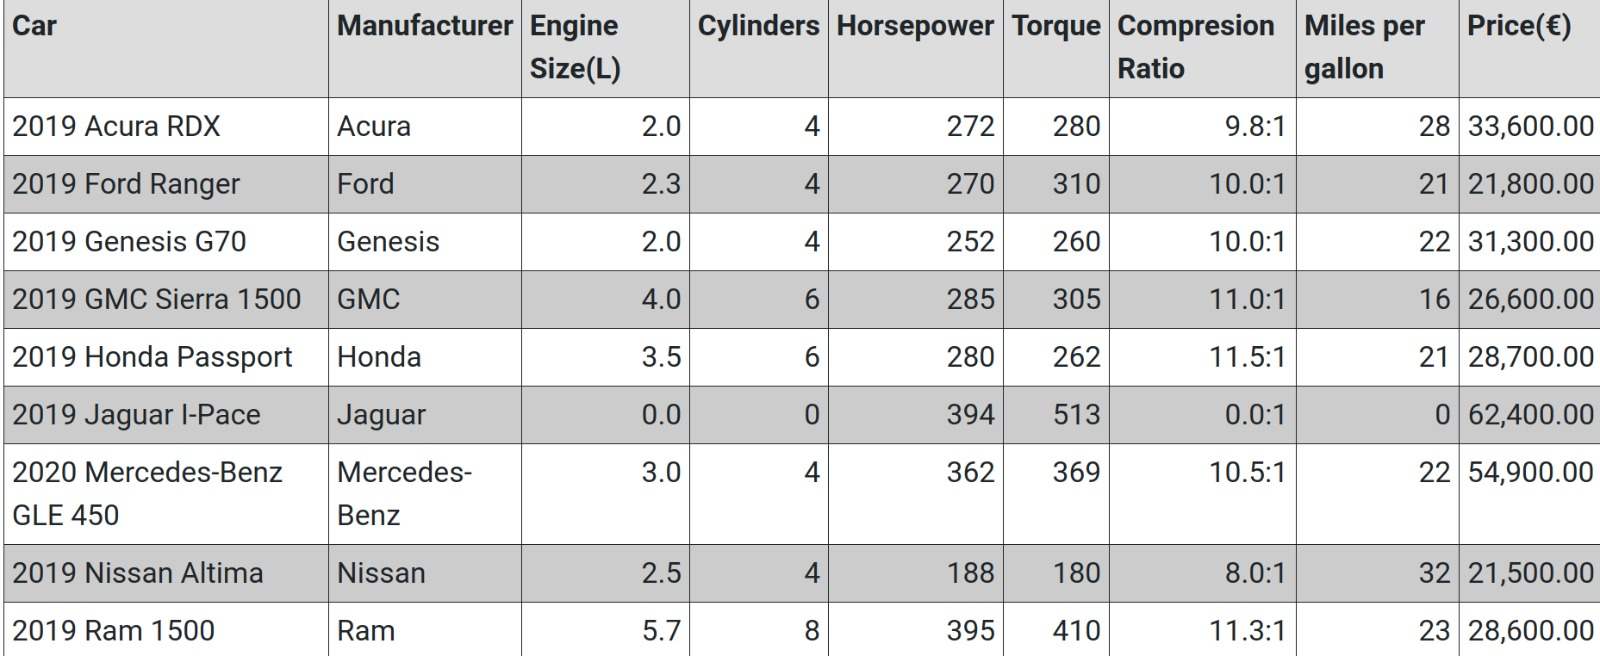
\includegraphics[width=\linewidth]
    {alt_t.jpeg}%
    \label{alig1}%
    }

    
    \caption[Alternate row highlighting]
    {
      
    \imgcredit{Screenshot taken by the author.}
    }
    \label{figWhol}
\end{figure}


\subsection{Current Row Highlighting}
Now again, talking about a big table, and going through it, one may 
easily becomes lost and wouldn't know in which row he is at the moment, which can be
pretty stressful. Again with the help of some CSS, the lives of the users' is made easier.

\begin{lstlisting}[%
    language = HTML, 
    xleftmargin=0cm,              % no extra margins for floats
    xrightmargin=0cm,             % no extra margins for floats
    language=biblatex,
    basicstyle=\footnotesize\ttfamily,
    frame=shadowbox,
    numbers=left,
    label=list:BibACMIEEE,
     stringstyle=\color{blue}
    ,
]
    % An example of using simple CSS to highlight table rows:

	table {
      overflow: hidden;
	}

	tr:hover {
	  background-color: #ffa;
	}

	td, th {
	  position: relative;
	}
	td:hover::after,
	th:hover::after {
	  content: "";
	  position: absolute;
	  background-color: #ffa;
	  left: 0;
	  width: 100%;
	  z-index: -1;
	}

\end{lstlisting}


\newpage

And again, it is shown how a small amount of CSS can be helpful.
The result:
\begin{figure}[H]
    \centering
  
    {%
    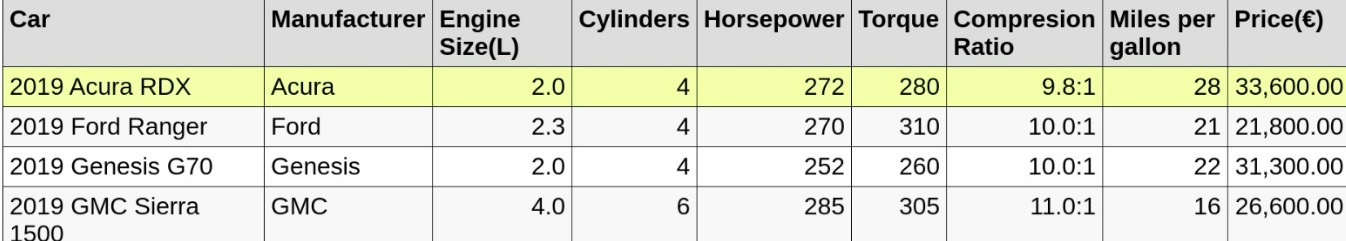
\includegraphics[width=\linewidth]
    {current_hl.jpeg}%
    \label{alig1}%
    }

    
    \caption[Current Row Highlighting]
    {
      
    \imgcredit{Screenshot taken by the author.}
    }
    \label{figWhol}
\end{figure}




\subsection{Pagination (With Sort and Search)}
The amount of data increases every second, over 2.5 quintillion bytes of data are made every day and there is also estimation that in 2020 will be created 1.7MB of data in every second for each person in the world. 
\newline 
Tables are sometimes one of the possible places for saving large sets of data.
This type of tables should consists of different types of features that enables users easier operations of maintaining.
\newline
Were the table be too long, we can divide it into 'pages'. We view a certain amount of rows at a time.
\newline

We provided this example of good table design with different features called pagination, because the most important feature of this technique is pagination.
With this feature is possible to determine the number of rows per page, previous  and next page navigation are also available. 
Every user has also possibility to filter results by text search and in this way find the desired row.
There is also possibility to sort table content in an descending or ascending order.

This solution works for following browsers:
\newline $\bullet$ Google Chrome
\newline $\bullet$ Mozzila Firefox
\newline $\bullet$ Internet Explorer
\newline $\bullet$ Opera
\newline $\bullet$ Microsoft Edge

For the implementation we used plug-in for the jQuery Javascript library called DataTables.


\begin{lstlisting}[%
    language = HTML, 
    xleftmargin=0cm,              % no extra margins for floats
    xrightmargin=0cm,             % no extra margins for floats
    language=biblatex,
    basicstyle=\footnotesize\ttfamily,
    frame=shadowbox,
    numbers=left,
    label=list:BibACMIEEE,
     stringstyle=\color{blue}
    ,
]
    % An example of using Javascript plugin DataTable():
    %Include these two files in order to include additional advanced features to any HTML table
    %cdn.datatables.net/1.10.20/css/jquery.dataTables.min.css
    %cdn.datatables.net/1.10.20/js/jquery.dataTables.min.js

    $(document).ready(function(){
        $('#myTable').dataTable(); //this plugin provides searching, sorting and pagination
 });

\end{lstlisting}

Table is initilaized with "myTable" id and this id is used in ready function() to assign dataTable funcionality to our HTML table instance. 

Following image represents html table with sorted Price column and 10/12 entries:
\begin{figure}[H]
    \centering
  
    {%
    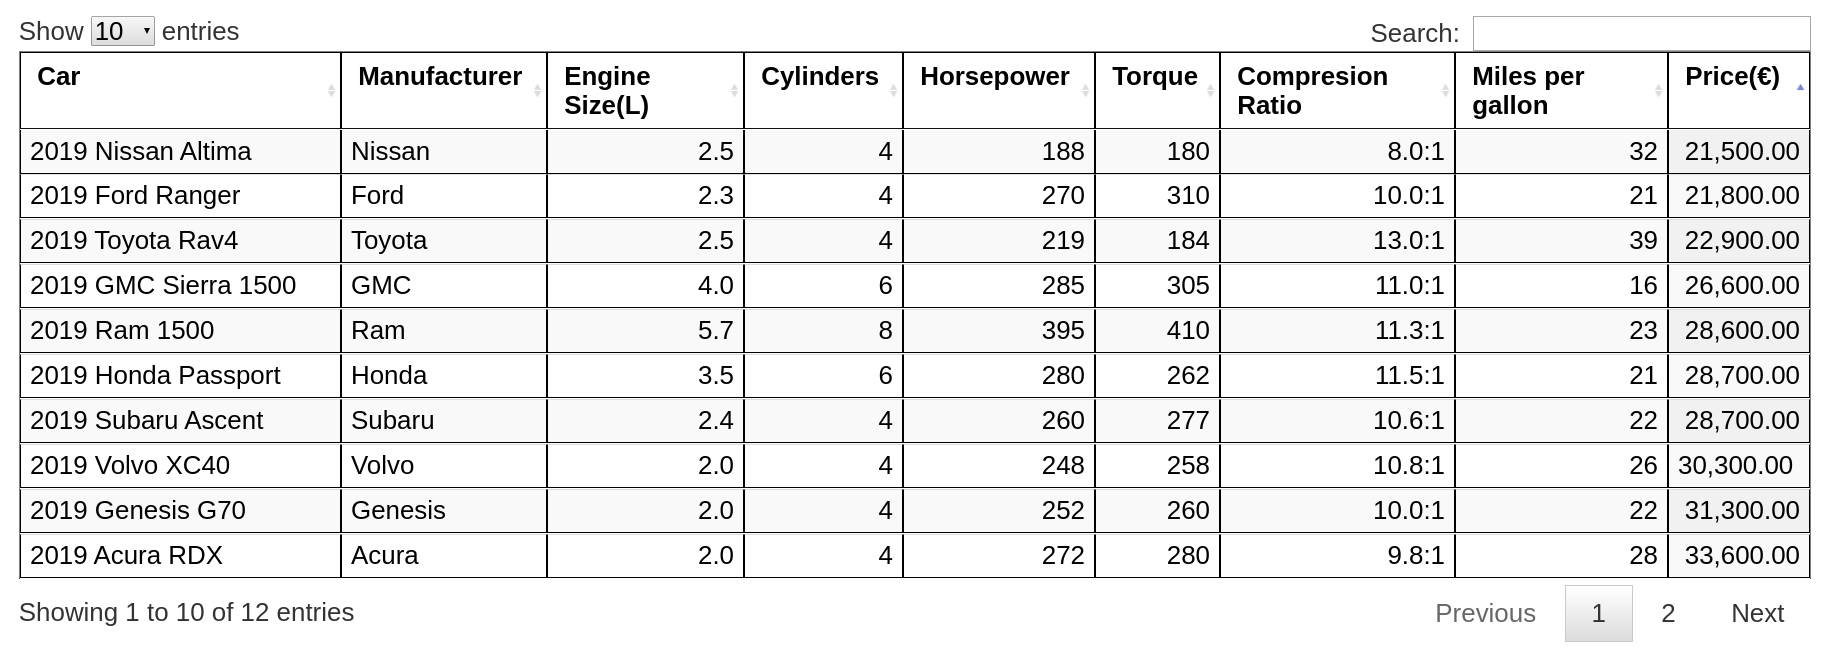
\includegraphics[width=\linewidth]
    {pagination_2.png}%
    \label{alig1}%
    }

    
    \caption[Pagination with sort option]
    {
      
    \imgcredit{Screenshot taken by the author.}
    }
    \label{figWhol}
\end{figure}

Following image represents html table with searched term:
\begin{figure}[H]
    \centering
  
    {%
    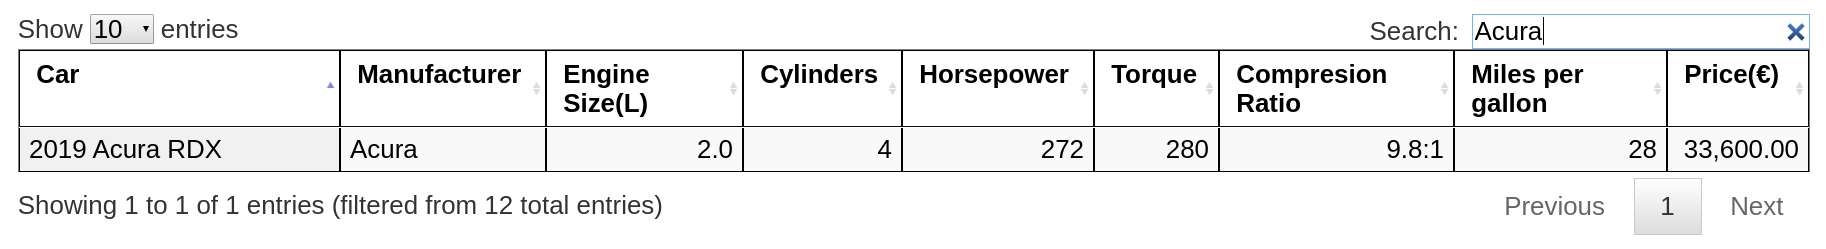
\includegraphics[width=\linewidth]
    {pagination_1.png}%
    \label{alig1}%
    }

    
    \caption[Pagination with search option]
    {
      
    \imgcredit{Screenshot taken by the author.}
    }
    \label{figWhol}
\end{figure}

\newpage

\section{Responsive Tables}

Data tables can contain many information, which makes displaying that data quite messy and hard to
look at. So by using responsive design, a big favor is done to the clients,
by adjusting the table according to their devices. One idea would be to minimize the table, but if the user is looking
at the table from his mobile device, he would have to zoom in, which is not that useful to him, because then again he would need to scroll
to view the whole table [9].

\begin{figure}[H]
    \centering
  
    {%
    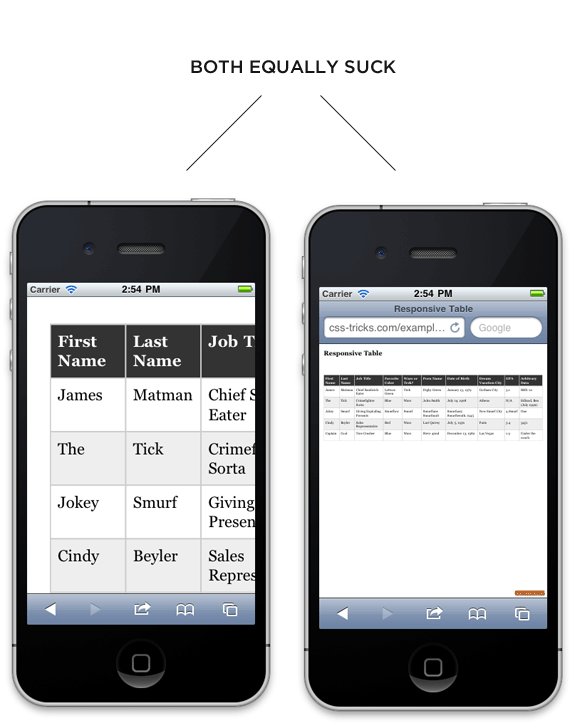
\includegraphics[width=\linewidth]
    {zoom_1.png}%
    \label{alig1}%
    }

    
    \caption[Before reponsive]
    {
      
    \imgcredit{https://css-tricks.com/responsive-data-tables/.}
    }
    \label{figWhol}
\end{figure}

As seen in the figure above, both options do not really look nor do as any good.
So, by using some simple CSS it is possible to fix that problem. With the help of the mentioned
media queries, it is possible to specify for which device sizes, which settings should be used. 

\begin{lstlisting}[%
    language = HTML, 
    xleftmargin=0cm,              % no extra margins for floats
    xrightmargin=0cm,             % no extra margins for floats
    language=biblatex,
    basicstyle=\footnotesize\ttfamily,
    frame=shadowbox,
    numbers=left,
    label=list:BibACMIEEE,
     stringstyle=\color{blue}
    ,
]
    % An example of using simple CSS with media queries on how to achieve Responsive Design:

    @media 
only screen and (max-width: 760px),
(min-device-width: 768px) and (max-device-width: 1024px)  {

	/* Force table to not be like tables anymore */
	table, thead, tbody, th, td, tr { 
		display: block; 
	}
	
	/* Hide table headers (but not display: none;, for accessibility) */
	thead tr { 
		position: absolute;
		top: -624.9375rem;
		left: -624.9375rem;
	}
	
	tr { border: 1px solid #ccc; }
	
	td { 
		/* Behave  like a "row" */
		border: none;
		border-bottom: 1px solid #eee; 
		position: relative;
		padding-left: 50%; 
	}
	
	td:before { 
		/* Now like a table header */
		position: absolute;
		/* Top/left values mimic padding */
		top: 0;
		left: 0.375rem;
		width: 45%;
		padding-right: 0.625rem;
		white-space: nowrap;
	}

\end{lstlisting}

\newpage
And now, the end result would be the following one:
\begin{figure}[H]
    \centering
  
    {%
    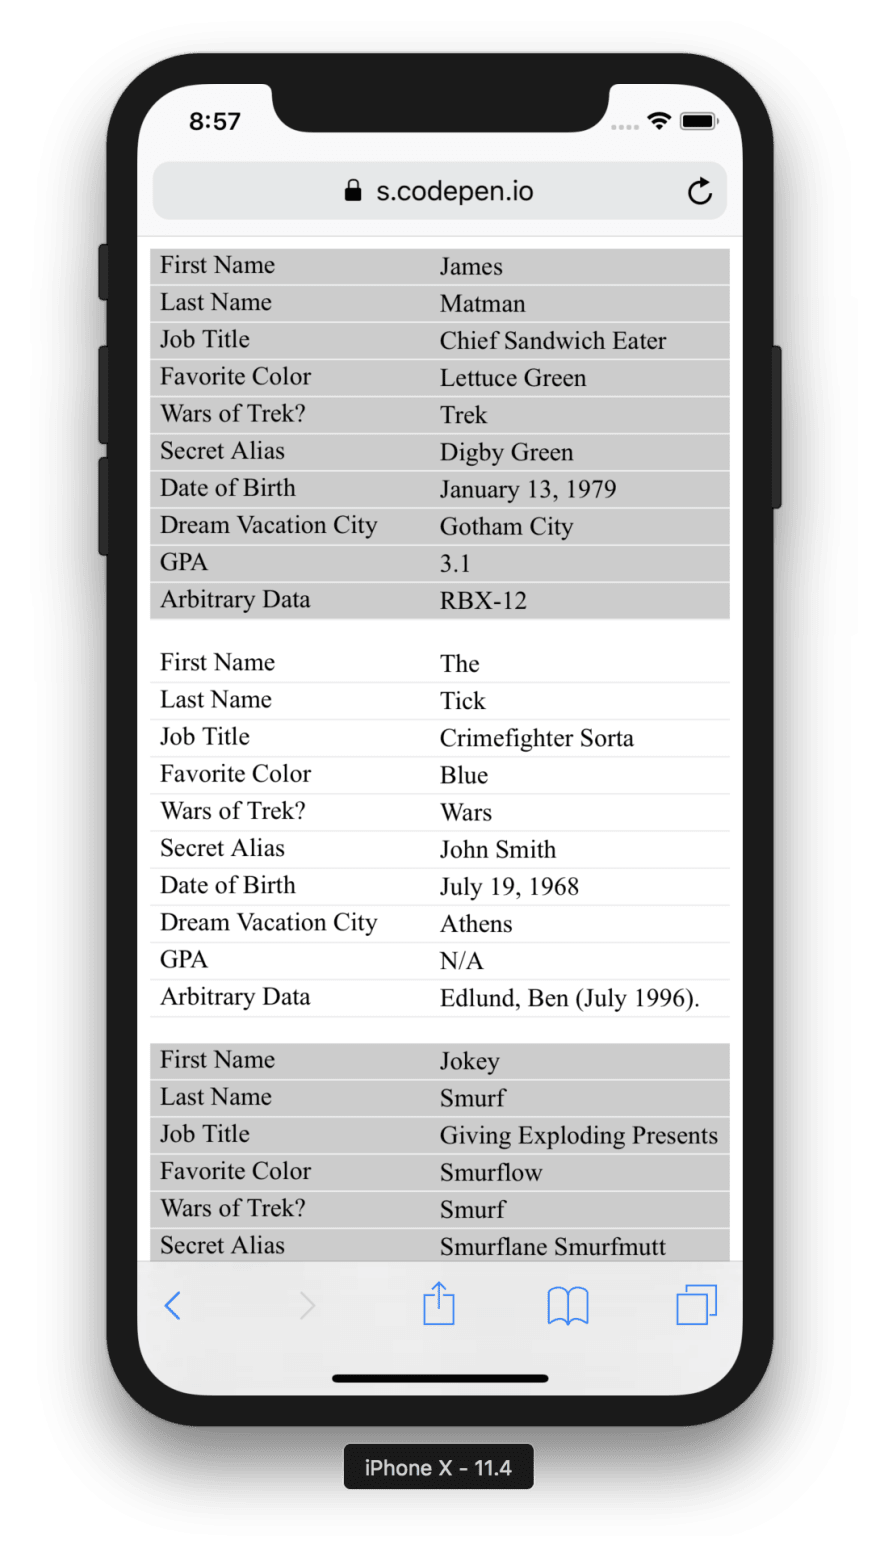
\includegraphics[width=0.45\linewidth]
    {zoom_3.png}%
    \label{alig1}%
    }

    
    \caption[After reposnsive]
    {
      
    \imgcredit{https://css-tricks.com/responsive-data-tables/.}
    }
    \label{figWhol}
\end{figure}


\subsection{Horizontal Scroll}
When the allocated space is too small - horizontally, instead of hiding it, we create a horizontal scroll bar just for the table and let the user scroll away. 
\newline 

Horizontal Scrolling represents a technique that resizes the table  
into columns at small screen resoultion. The rows can be scrolled from left to right with fixed first row.
This is different from viewport scrolling as we scroll only through the table.
\newline 

It is very useful technique when presenting large data sets with identifiers in the first column. Then is very easy for every user to compare data content with multiple identifiers.


This solution works for following browsers:
\newline $\bullet$ Google Chrome
\newline $\bullet$ Mozzila Firefox
\newline $\bullet$ Internet Explorer
\newline $\bullet$ Opera
\newline $\bullet$ Microsoft Edge
\newline
\newline It is impossible to find one size that fits all solution. Data comparing is very difficult on the small screens.
There are a lot of possible workarounds for this issue, but no one can solve this problem. 
Our implementation of horizontal scrolling creates table elements scrollable, but also can not solve the issue to the end.
We will explain all important css-properties that creates a responsive table with horizontal scrolling.

\begin{lstlisting}[%
    language = HTML, 
    xleftmargin=0cm,              % no extra margins for floats
    xrightmargin=0cm,             % no extra margins for floats
    language=biblatex,
    basicstyle=\footnotesize\ttfamily,
    frame=shadowbox,
    numbers=left,
    label=list:BibACMIEEE,
     stringstyle=\color{blue}
    ,
]
.rtable {

    display: inline-block;
    vertical-align: top;
    max-width: 100%;

    overflow-x: auto;

    // optional - looks better for small cell values
    white-space: nowrap;

    border-collapse: collapse;
    border-spacing: 0;
}

\end{lstlisting}

This css code represents css class .rtable used in the case when container is not resized.
With display: inline-block all items are listed horizontally instead of vertically.
Vertical-align property maintains how elements set next to each other in a line.
The overflow property determines whether to crop content or to add scroll bars (along the x-axis) when a table's content is too big to satisfy some screen resolution.
We can use white-space: nowrap property as optional for small cell values.
Css border properties are used to control borders into a table.  

Following image represents html table with horizontal scroll:

\begin{figure}[H]
    \centering
  
    {%
    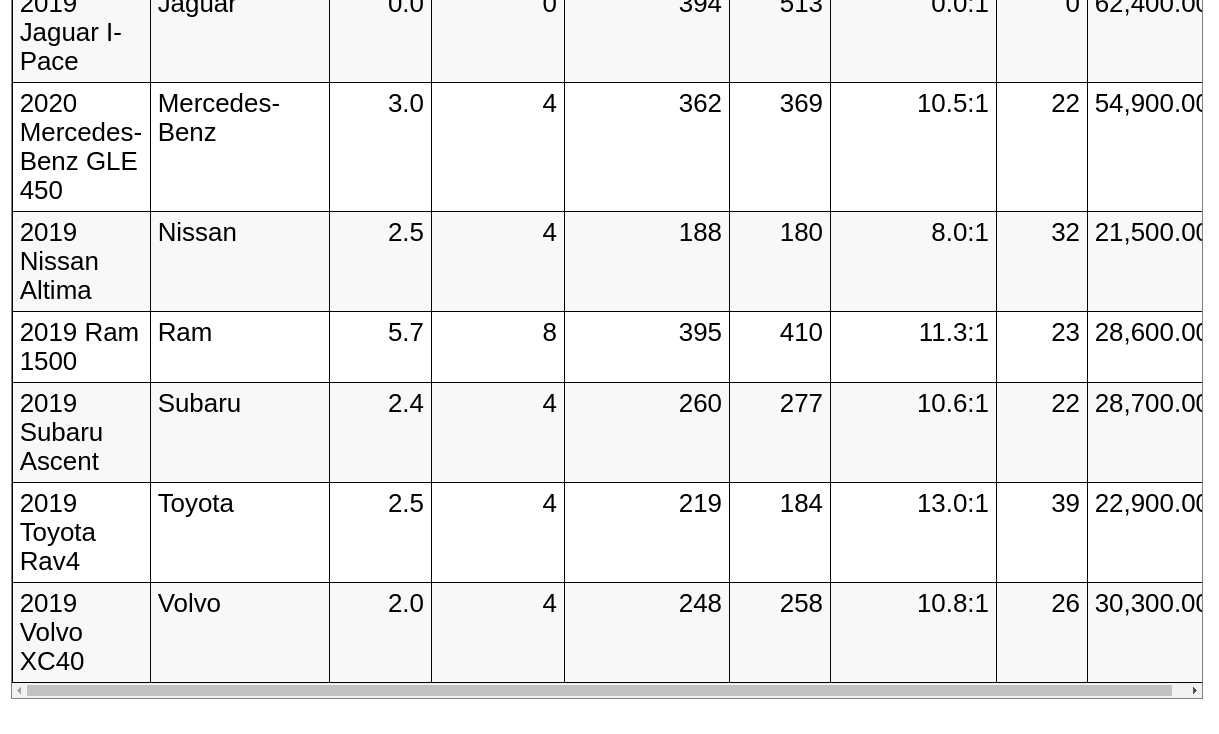
\includegraphics[width=1\linewidth]
    {horizontal.png}%
    \label{alig1}%
    }

    
    \caption[Horizontal Scroll]
    {
      
    \imgcredit{Screenshot taken by the author.}
    }
    \label{figWhol}
\end{figure}


\subsection{Fixed Header}
When the table is vertically long, we fix the table's header to the top of the table's view.
As we scroll down, we keep the table's header always visible.
\newline

It is very useful to have the fixed header (first row fixed) on the top of the table, when presenting tables with a particularly larage data set. 
This helps users to quickly determine what every column identify rather than need to scroll back to the top of the table every time. 
\newline Fixed Header provides background on what column the user is on.
This is very effective feature that makes our life easier.

This solution works for following browsers:
\newline $\bullet$ Google Chrome
\newline $\bullet$ Mozzila Firefox
\newline $\bullet$ Internet Explorer
\newline $\bullet$ Opera
\newline $\bullet$ Microsoft Edge

\begin{lstlisting}[%
    language = HTML, 
    xleftmargin=0cm,              % no extra margins for floats
    xrightmargin=0cm,             % no extra margins for floats
    language=biblatex,
    basicstyle=\footnotesize\ttfamily,
    frame=shadowbox,
    numbers=left,
    label=list:BibACMIEEE,
     stringstyle=\color{blue}
    ,
]
.fixedHeader tbody {
    display: block;
    overflow: auto;
    width: 100%;
}

.fixedHeader thead tr {
    display: table;
    width: 100%;
    table-layout: fixed;
}

.fixedHeader thead, .fixedHeader tbody tr {
    display: table;
    width: 100%;
    table-layout: fixed;
}

.fixedHeader thead {
    width: calc( 100% - 0.6em )
}

.fixedHeader td {
    width: 100%;
}

\end{lstlisting}

Tbody element is determined with the type of rendering box. 
With overflow: auto scrollbar will appear along y-axis.
All thead and tbody rows will behave as table elements.
Fixed table layout algorithm is used to control table and column widths.
Width for almost every table element is static, just the header has non-static width.
The width of header is determined with calc() function and in this way is solved the main issue in this responsive technique.

Following image represents html table with fixed header:

\begin{figure}[H]
    \centering
  
    {%
    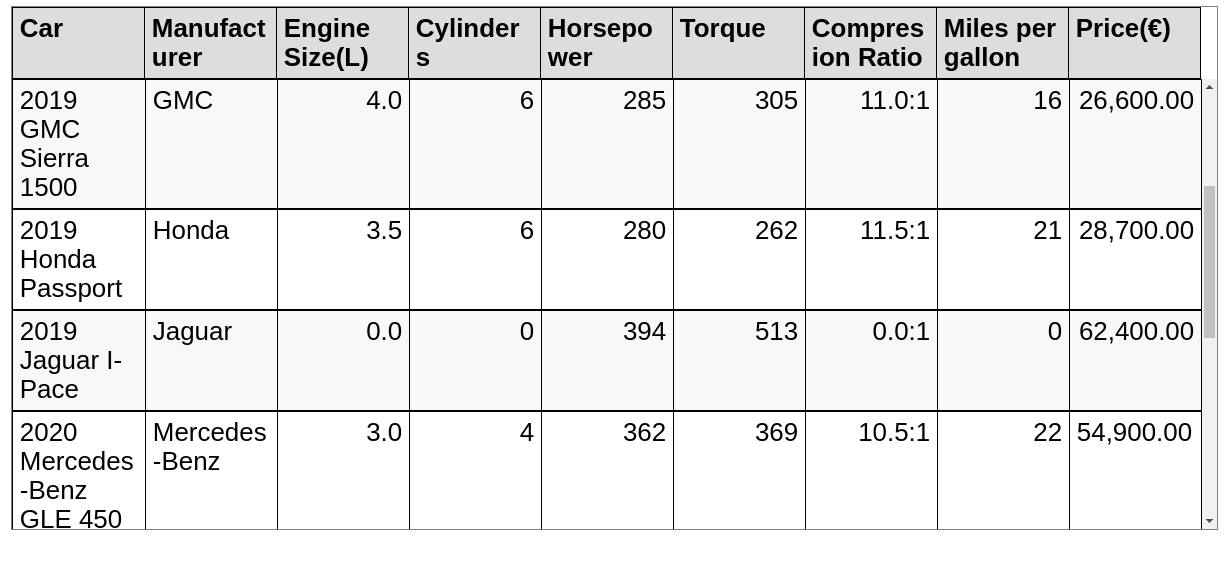
\includegraphics[width=1\linewidth]
    {fixed_header.png}%
    \label{alig1}%
    }

    
    \caption[Fixed Header]
    {
      
    \imgcredit{Screenshot taken by the author.}
    }
    \label{figWhol}
\end{figure}
